\documentclass[aspectratio=169, xcolor=table]{beamer}

\usepackage{textcomp}       % Text companion fonts
\usepackage{tikz}           % Powerful drawing package, part of pgf
\usepackage{graphbox}       % For centre alignment of graphics

\setbeamertemplate{navigation symbols}{}
\setbeamertemplate{items}[circle]

\hyphenpenalty 4000 \sloppy

% PGF and TikZ definitions for this paper

% TikZ library imports
\usetikzlibrary{positioning}        % Anchor placement support
\usetikzlibrary{calc}               % Coordinate calculations
\usetikzlibrary{shapes.geometric}   % cylinder
\usetikzlibrary{shapes.arrows}      % arrow shapes
\usetikzlibrary{shapes.multipart}
\usetikzlibrary{shapes.symbols}
\usetikzlibrary{fit}                % Fitting outline to shape
\usetikzlibrary{arrows}
\usetikzlibrary{arrows.meta}
\usetikzlibrary{shadows}
\usetikzlibrary{spy}


% Define our colours
\colorlet{normal colour}{green!60!blue!20}  % Normal coloured filled areas
\colorlet{accent colour}{orange!25}         % Accented filled areas
\colorlet{background colour}{black!10}      % Background groups
\colorlet{data colour}{black!50}            % Data flow
\colorlet{trigger colour}{black!80}         % Trigger lines
\colorlet{control colour}{blue!50}          % Other lines etc


% Common TikZ definitions
\tikzset{
    % This seems a reasonably comfortable arrow shape
    >=stealth,
%
    % Define a set of styles
    % First some fills
    background fill/.style={fill=background colour},
    highlight fill/.style={fill=normal colour},
    accent fill/.style={fill=accent colour},
    % Next some lines
    bus/.style={draw, color=data colour, text=black, line width=0.6mm, ->},
    control/.style={color=control colour, text=black, very thick, ->},
%
    % Used for creating an exact fit to an existing list of objects
    tight fit/.style={fit=#1, inner sep=0, line width=0},
    % We almost always want centre aligned node text
    every node/.style={align=center},
%
    box/.style={
        draw, rectangle, very thick, highlight fill,
        minimum width=1.5cm, minimum height=1.1cm},
    small box/.style={
        draw, rectangle, thick, highlight fill},
    component/.style={
        draw, rectangle, thick, accent fill,
        minimum width=11mm, minimum height=8mm},
    buffer/.style={
        regular polygon, regular polygon sides=3, anchor=center,
        accent fill, thick, draw},
    generate/.style={
        background fill, thin, draw=gray,
        copy shadow={
            shadow xshift=1ex, shadow yshift=-1ex}},
%
    small label/.style={anchor=south west, inner sep=2pt, font=\small},
%
    trigger line/.style={thin, trigger colour},
    trigger/.style={
        trigger line, >={Triangle[open, scale=1.2]}, shorten >=-5pt, ->},
    trigger dot/.style={fill, circle, inner sep=1pt, line width=-1pt},
    mul/.style={
        draw=black, circle, thick, highlight fill, inner sep=0.5ex},
%
    inline text/.style={
        baseline=(current bounding box.base),
        every node/.append style={anchor=base, font=\scriptsize},},
%
    pics/buffer/.style args={#1/#2}{
        code={
            \draw [thick, -, black] (0.5mm,-2mm) -- (0.5mm,2mm);
            \draw [thick, -, black] (-0.5mm,-2mm) -- (-0.5mm,2mm);
            \node at (0,2mm) [
                rotated anchor=-90, font=\scriptsize, inner sep=0.2em] {#1}
            node at (0,-2mm) [
                rotated anchor=90, font=\scriptsize, inner sep=0.2em] {#2};}},
%
% A helper for drawing ADC and DAC symbols
    adc-dac/.style={
        draw, thick, accent fill, signal, signal to=#1,
        minimum height=8mm, signal pointer angle=120
    },
}


% New tikz key definitions to control behaviour of \multipath.
\tikzset{
    % Default colour for multipath background
    multipath background/.initial=white,
    multipath margin/.initial=0.3mm,
}

% Draws multiple paths with an outline on each path.  Call with path options as
% first optional argument and with a list of paths as the second argument.
\newcommand{\multipath}[2][]{
    \begin{scope}[#1]
        % Pick up multipath margin and background definitions
        \newcommand{\margin}{\pgfkeysvalueof{/tikz/multipath margin}}
        \newcommand{\background}{\pgfkeysvalueof{/tikz/multipath background}}

        % Draw a white background a bit larger than the programmed line
        % thickness.  We turn off any arrows and shorten the line a trifle to
        % avoid any erosion of the endpoints.
        \begin{scope}[
            line width=\pgflinewidth+\margin, color=\background,
            shorten >=\margin, shorten <=\margin, -]
        #2
        \end{scope}

        % Now draw the target path with its original options.
        #2
    \end{scope}
}

% Special coordinates along edge of box
\newcommand{\northcoord}[3]{
    \coordinate (#1 #2) at ($(#1.north west)!#3!(#1.north east)$)}
\newcommand{\eastcoord}[3]{
    \coordinate (#1 #2) at ($(#1.south east)!#3!(#1.north east)$)}
\newcommand{\southcoord}[3]{
    \coordinate (#1 #2) at ($(#1.south west)!#3!(#1.south east)$)}
\newcommand{\westcoord}[3]{
    \coordinate (#1 #2) at ($(#1.south west)!#3!(#1.north west)$)}


% Trick for reusing last coordinate
\makeatletter
\newcommand\lastcoord{\the\tikz@lastxsaved,\the\tikz@lastysaved}
\makeatother


% It's convenient to have a background layer
\pgfdeclarelayer{background}
\pgfsetlayers{background,main}


% Useful for inline boxes
\newcommand\smallbox[2][small box]{\tikz [inline text] \node [#1] {#2};}


% ------------------------------------------------------------------------------
% This frightening looking code is used to compute an anchor that rotates with
% the entire picture.  This is useful when anchoring a node in a pic that itself
% will be rotated.
%   Some really tricky code taken from stack overflow question here:
%
%   https://tex.stackexchange.com/questions/128565/
%       how-to-allow-labels-anchors-in-tikz-to-be-affected-by-
%       rotations-without-rotatin

% \pgfmath@smuggleone
%
% Smuggle a macro outside a group.
%
% Changed by TT: Speedup by insisting, that smuggleone is directly
% followed by \endgroup
%
\makeatletter
\def\pgfmath@smuggleone#1\endgroup{%
  \expandafter\endgroup\expandafter\def\expandafter#1\expandafter{#1}}

\let\pgfmathsmuggle=\pgfmath@smuggleone
\makeatother

\tikzset{
    rotated anchor/.code=%
        \begingroup
            \pgfcoordinate{qrr@origin}{\pgfpointorigin}%
            \pgfcoordinate{qrr@direct}{\pgfpointpolarxy{#1}{1}}%
            \pgftransformreset
            \pgfmathanglebetweenpoints{%
                \pgfpointanchor{qrr@origin}{center}}{%
                    \pgfpointanchor{qrr@direct}{center}}%
            \pgfmathsmuggle\pgfmathresult
        \endgroup
    \tikzset{anchor/.expanded=\pgfmathresult}%
}

% ------------------------------------------------------------------------------

% vim: set filetype=tex:


% Some commands for colouring tables
\newcommand{\cg}{\cellcolor{green!60!blue!20}}
\newcommand{\cy}{\cellcolor{yellow}}
\newcommand{\co}{\cellcolor{orange!40!yellow}}

\newcommand{\re}{\operatorname{re}}
\newcommand{\im}{\operatorname{im}}
\newcommand{\R}{\mathbb{R}}

\title{%
    Tune Computation via Model Fitting\\to Swept Machine Response Measurement}
\author{Michael Abbott}
\date{IBIC 2019}
\institute{Diamond Light Source}


\begin{document}


% ------------------------------------------------------------------------------
%
\begin{frame}
\titlepage
\end{frame}

\setbeamertemplate{footline}{%
    \vspace*{-8pt}\hspace*{2pt}%
    Tune Computation via Model Fitting to Swept Machine Response Measurement,
    IBIC 2019 \hfill \insertpagenumber\hspace*{2pt}
}


% ------------------------------------------------------------------------------
%
\begin{frame}{Overview of Talk}

\begin{itemize}
\item Response measurement (\emph{Beam Transfer Function}):

Using multi-bunch feedback system as vector network analyser.

\item Multi-pole resonator model:

Note that this is \emph{not} a machine physics model.
\item Fitting the model, finding the tune:

Python code for fitter available from author.
\item Complications!

Fitting doesn't always work, some sweeps are hard to interpret.
\end{itemize}

\end{frame}


% ------------------------------------------------------------------------------
%
\begin{frame}{Overview of Tune Measurement Process}
\begin{tikzpicture}[
    start chain, node distance=1mm]

\path
    node [on chain] (orbit-view) {%
        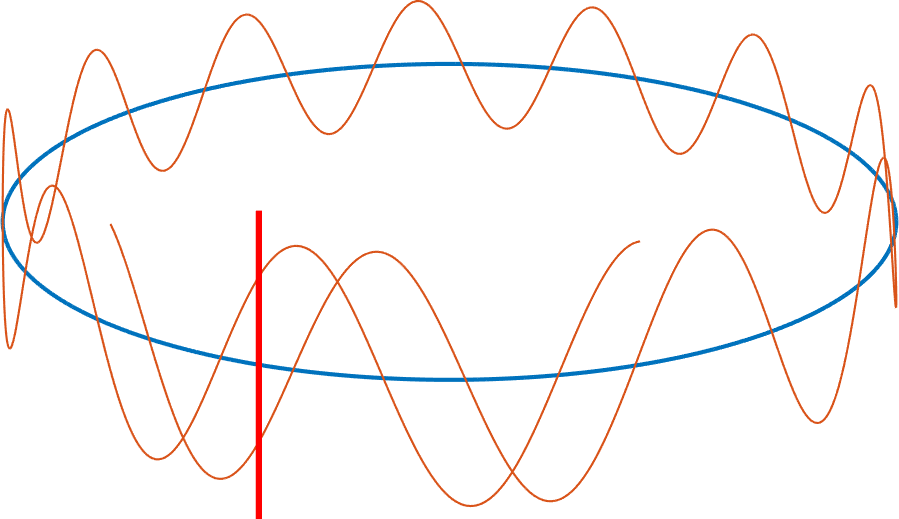
\includegraphics[width=3.2cm]{orbit-view.png}}
    node [anchor=south, text width=4cm] at (orbit-view.north) {%
        Machine Betatron and Synchrotron Tunes}

    node [anchor=north, text width=4cm] at (orbit-view.south) {%
        \small Tune excitation and measurement at a single location.}

    node [on chain, single arrow, draw, minimum height=0.6cm] {}

    node [on chain] (raw) [text width=3.5cm] {}
    node [anchor=south, label={above:\small Measured Magnitude}] at (raw) {%
        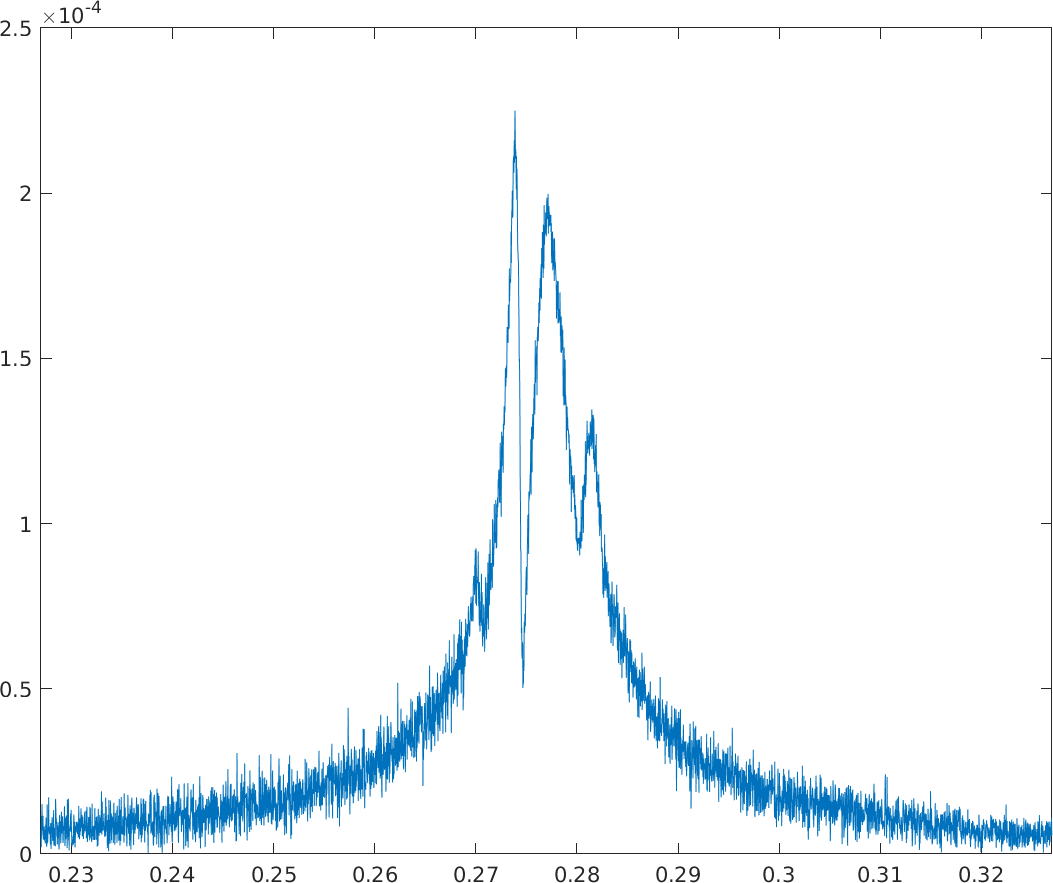
\includegraphics[width=3.5cm]{raw-iq-power.png}}
    node [anchor=north, label={below:\small Measured IQ}] at (raw) {%
        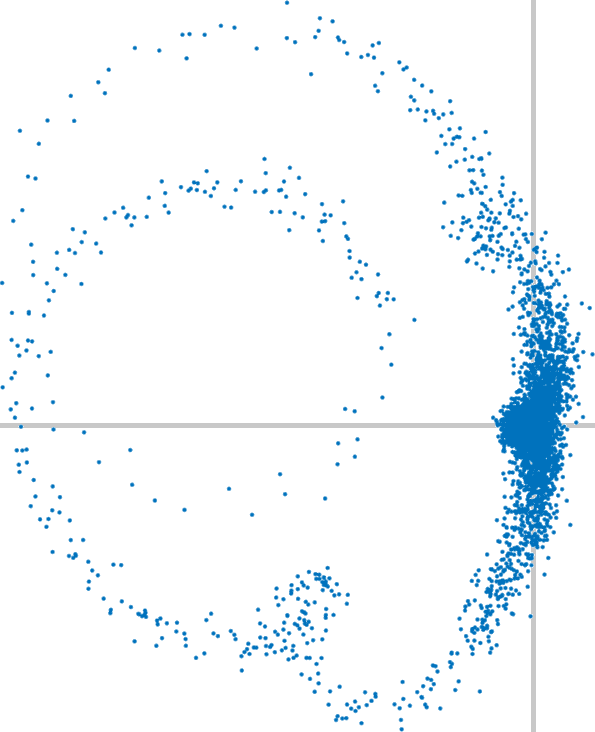
\includegraphics[width=2cm]{raw-iq.png}}

    node [on chain, single arrow, draw, minimum height=0.6cm] {}

    node [on chain, yshift=1.2cm] (fitted) {%
        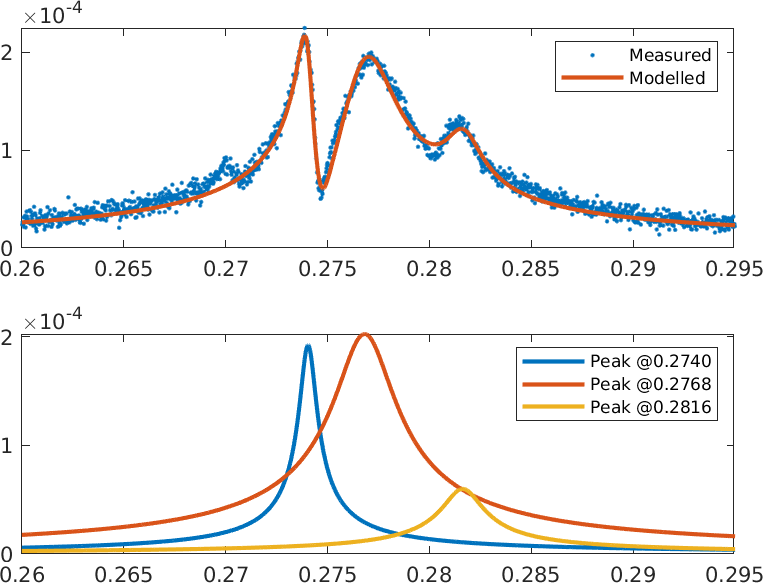
\includegraphics[width=4.5cm]{fitted-power.png}}
    node [anchor=south, text width=5cm] at (fitted.north) {%
        Model fitted to tune sweep}

    [continue chain=going below, node distance=5mm]
    node [on chain,
        single arrow, draw, minimum height=0.6cm,
        rotate=-90, anchor=center] {}

    node [on chain, very thick, draw=red, shift={(4mm,-2mm)},
        label={below:\small Tune Measurement}] {
        Tune = 0.2768\\Phase = 159\textdegree}
    ;

\end{tikzpicture}

% vim: filetype=tex:

\end{frame}


% ------------------------------------------------------------------------------
%
\begin{frame}{Measuring Beam Frequency Response}

\begin{centering}
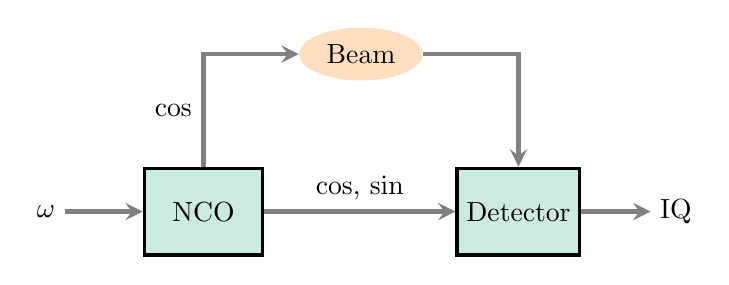
\begin{tikzpicture}[x=20mm, y=20mm]

\path
    (0,0) node [box] (nco) {NCO}
    +(-1,0) node (f) {$\omega$}
    (1,1) node [accent fill, ellipse] (beam) {Beam}
    (2,0) node [box] (detector) {Detector}
    +(1,0) node (iq) {IQ};

\draw [bus] (f) -- (nco);
\draw [bus] (nco) |- (beam) node [pos=0.25, left] {cos};
\draw [bus] (beam) -| (detector);
\draw [bus] (nco) -- (detector) node [midway, above] {cos, sin};
\draw [bus] (detector) -- (iq);

\end{tikzpicture}

% vim: filetype=tex:

\end{centering}

\bigskip

By exciting the beam at a selected frequency $\omega$ and measuring the response
of the beam at that frequency, we compute the \emph{transfer function} of the
machine at the selected frequency:

\begin{equation*}
    R(\omega) = \sum_{t\in\text{dwell}(\omega)} e^{-i \omega t} x_t
\end{equation*}

This can be expressed as phase and magnitude, or equivalently as a
complex number, or in digital processing terms as a pair (I,Q).

\end{frame}


% ------------------------------------------------------------------------------
%
\begin{frame}{System Setup for Bunch-by-Bunch Control}

\tikzset{
    actuator/.style={circle, inner sep=1pt, highlight fill, draw=black}}

\begin{centering}
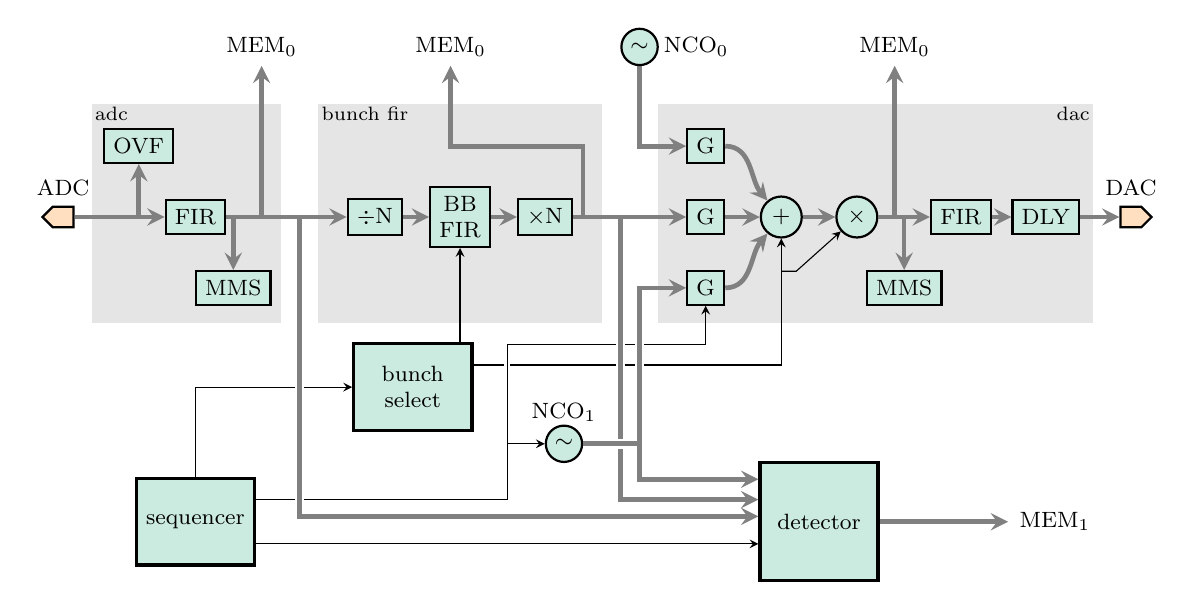
\begin{tikzpicture}[
    adc-dac/.style={
        draw, single arrow, thick, accent fill,
        single arrow head extend=0pt, shape border rotate=#1},
    area label/.style={anchor=north west, font=\scriptsize, inner sep=1pt},
    mul/.style={
        draw=black, circle, thick, highlight fill, inner sep=0.5ex},
    every node/.append style={font=\footnotesize},
    control mux/.style={
        small box, accent fill, label={[font=\tiny]above:MUX}, font=\tiny},
    x=12mm, y=9mm
    ]

    \path [background fill] (0.3,1.6)
        node [area label] {adc} rectangle ++(2,-3.1);
    \path [background fill] (2.7,1.6)
        node [area label] {bunch fir} rectangle ++(3.0,-3.1);
    \path [background fill] (6.3,1.6) rectangle ++(4.6,-3.1)
        ++(0,3.1) node [area label, anchor=north east] {dac};

    \path
        (0,0) node [adc-dac=180, label={ADC}] (adc in) {}
        +(0.8,1) node [small box] (adc ovf) {OVF}
        ++(1.4,0) node [small box] (adc fir) {FIR}
        +(0.4,-1) node [small box] (adc mms) {MMS}
        +(0.7,2.4) node (adc mem) {MEM\textsubscript{0}}
        ++(1.9,0) node [small box] (decimate) {$\div$N}
        ++(0.9,0) node [small box] (bb fir) {BB\\FIR}
        ++(0.9,0) node [small box] (interpolate) {$\times$N}
        +(-1,2.4) node (fir mem) {MEM\textsubscript{0}}
        ++(1.7,0) node [small box] (fir gain) {G}
        +(0,1) node [small box] (nco0 gain) {G}
        +(0,-1) node [small box] (nco1 gain) {G}
        ++(0.8,0) node [mul] (sum) {$+$}
        ++(0.8,0) node [mul] (product) {$\times$}
        +(0.5,-1) node [small box] (dac mms) {MMS}
        +(0.4,2.4) node (dac mem) {MEM\textsubscript{0}}
        ++(1.1,0) node [small box] (dac fir) {FIR}
        ++(0.9,0) node [small box] (delay) {DLY}
        ++(0.9,0) node [adc-dac, label={DAC}] (dac out) {};

    \node [box] at (1.4,-4.3) (sequencer) {sequencer};
    \path (bb fir) ++(-0.5,-2.4) node [box] (bunch) {bunch\\select};
    \node [box, minimum height=15mm] at (8,-4.3) (detector) {detector};
    \path (nco1 gain) ++(-1.5,-2.2)
        node [mul,
            label={[inner sep=1pt]above:NCO\textsubscript{1}}] (nco1) {$\sim$};

    \draw [bus] (adc in) -- (adc fir);
    \draw [bus] (adc in) -| (adc ovf);
    \draw [bus] (adc fir) -| (adc mms);
    \draw [bus] (adc fir) -| (adc mem);
    \draw [bus] (adc fir) -- (decimate);

    \draw [bus] (decimate) -- (bb fir);
    \draw [bus] (bb fir) -- (interpolate);
    \draw [bus] (interpolate) -- (fir gain);
    \draw [bus] (interpolate) ++(0.4,0) -- ++(0,1) -| (fir mem);
    \draw [bus] (fir gain) -- (sum);
    \draw [bus] (nco0 gain) to [out=0, in=130] (sum);
    \draw [bus] (nco1 gain) to [out=0, in=-130] (sum);
    \draw [bus] (sum) -- (product);
    \draw [bus] (product) -- (dac fir);
    \draw [bus] (product) -| (dac mms);
    \draw [bus] (product) -| (dac mem);
    \draw [bus] (dac fir) -- (delay);
    \draw [bus] (delay) -- (dac out);

    \draw [bus, <-] (nco0 gain) -- ++(-0.7,0) -- ++(0,1.4)
        node [mul, label={[inner sep=1pt]right:NCO\textsubscript{0}}] {$\sim$};

    \draw [thin, ->] (sequencer) |- (bunch);
    \draw [thin, ->] (bunch.north-|bb fir) -- (bb fir);
    \draw [thin, <-] (product) -- ++(-130:1) -- (\lastcoord-|sum);
    \draw [thin, ->] (bunch.20) -| (sum);
    \draw [thin, ->] (sequencer.-20) -- (\lastcoord-|detector.west);
    \draw [thin, ->] (sequencer.20) -| ($(nco1)+(-0.6,0)$)
        coordinate (nco1 control) -- (nco1);
    \multipath [thin] {\draw (nco1 control) -- ++(0,1.4);}
    \draw [thin, ->] (nco1 control) -- ++(0,1.4) -| (nco1 gain);

    \multipath [bus] {\draw (interpolate) ++(0.8,0) |- (detector.160);}
    \multipath [bus] {\draw (adc fir) ++(1.1,0) |- (detector.175);}
    \multipath [bus, -] {
        \draw (nco1) -- ++(0.8,0) -- (\lastcoord|-nco1 gain);
        \draw (nco1) -- ++(0.8,0) -- (\lastcoord|-detector.145);
    }
    \draw [bus] (nco1) ++(0.8,0) |- (nco1 gain);
    \draw [bus] (nco1) ++(0.8,0) |- (detector.145);

    \draw [bus] (detector) -- ++(2,0)
        node [anchor=west] {MEM\textsubscript{1}};

\end{tikzpicture}

% vim: filetype=tex:

\end{centering}

\bigskip
\smallbox[actuator]{B} EBPM pickup;
\smallbox[actuator]{C} Longitudinal cavity;
\smallbox[actuator]{S} Transverse striplines.

\end{frame}


% ------------------------------------------------------------------------------
%
\begin{frame}{Typical Machine Response Measurement}

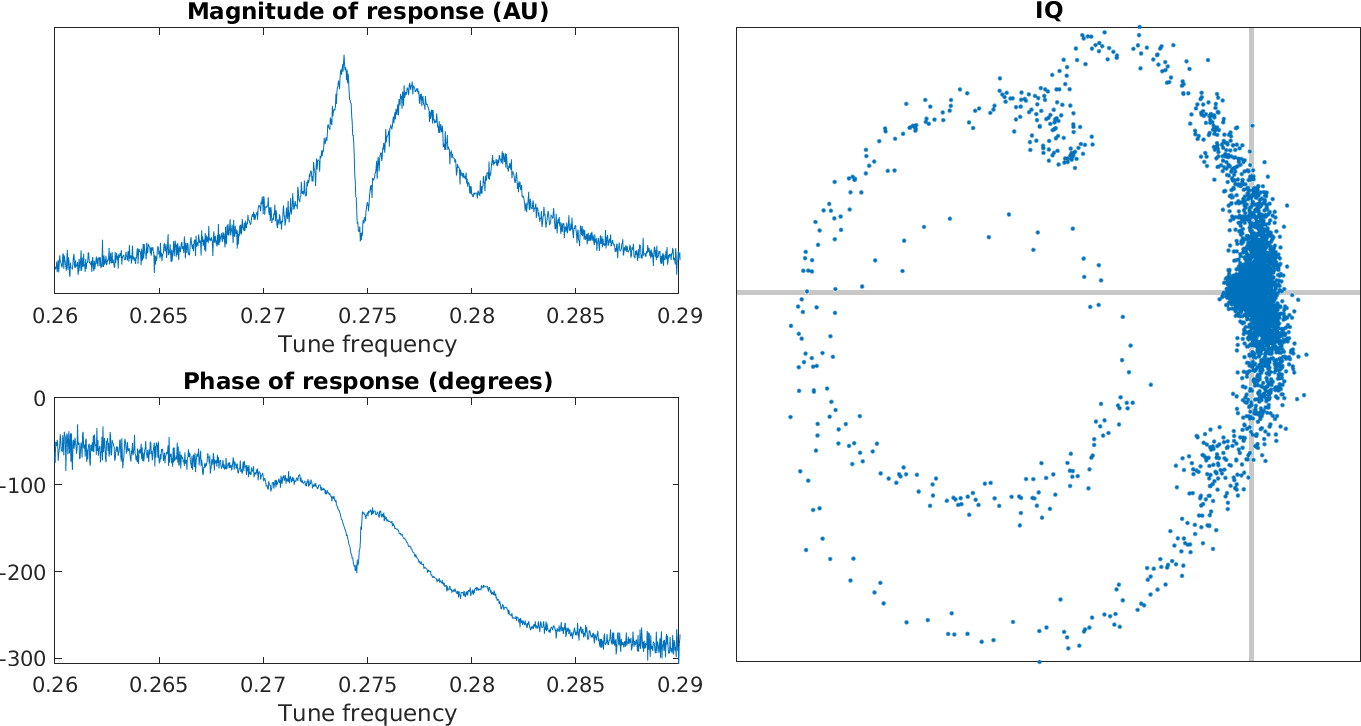
\includegraphics[width=0.95\linewidth]{typical-sweep.png}


\end{frame}


% ------------------------------------------------------------------------------
%
\begin{frame}{Damped Harmonic Oscillator}

\raisebox{0.5\height}{
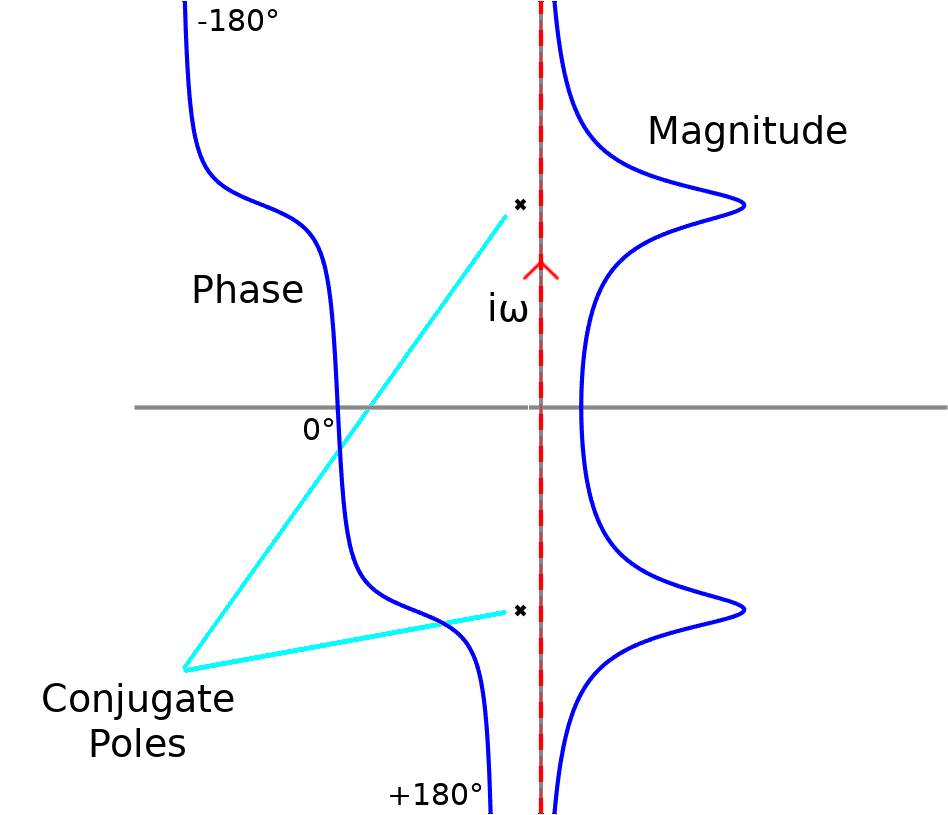
\includegraphics[width=0.45\linewidth]{pole-model.png}}%
\quad
%
\begin{overlayarea}{0.5\textwidth}{\textheight}
\only<1>{
\smallskip
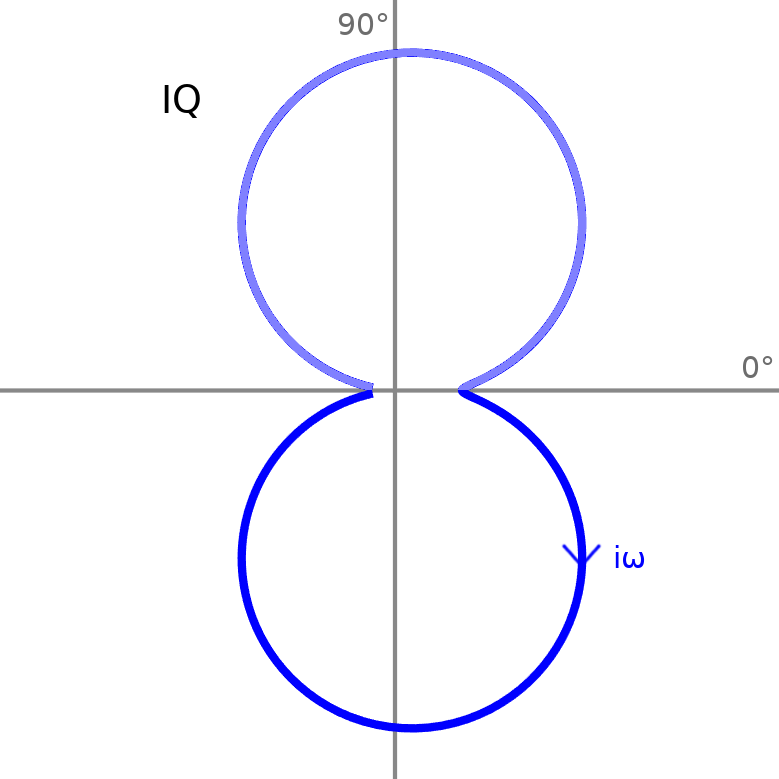
\includegraphics[width=0.86\linewidth]{two-pole-iq.png}%
}%
%
\only<2>{
Damped harmonic oscillator:
\[
    \ddot x + 2 \nu \dot x + \omega_0^2 x = y
\]

Laplace transform:
\[
    s^2 X + 2 \nu s X + \omega_0^2 X = Y
\]

Response:
\[
    \frac XY = \frac{1}{(s-b)(s-b^*)} =
    \frac{a}{s-b} - \frac{a}{s-b^*}
\]
where
\scriptsize{
\[
    a = \frac 1{2i\omega_c}\;, \quad
    b = \nu + i\omega_c\;, \quad
    \omega_c^2 = \omega_0^2 - \nu^2\;.
\]
}}
\end{overlayarea}

\end{frame}


% ------------------------------------------------------------------------------
%
\begin{frame}{Single Pole Resonator Model}

\begin{minipage}{0.45\textwidth}
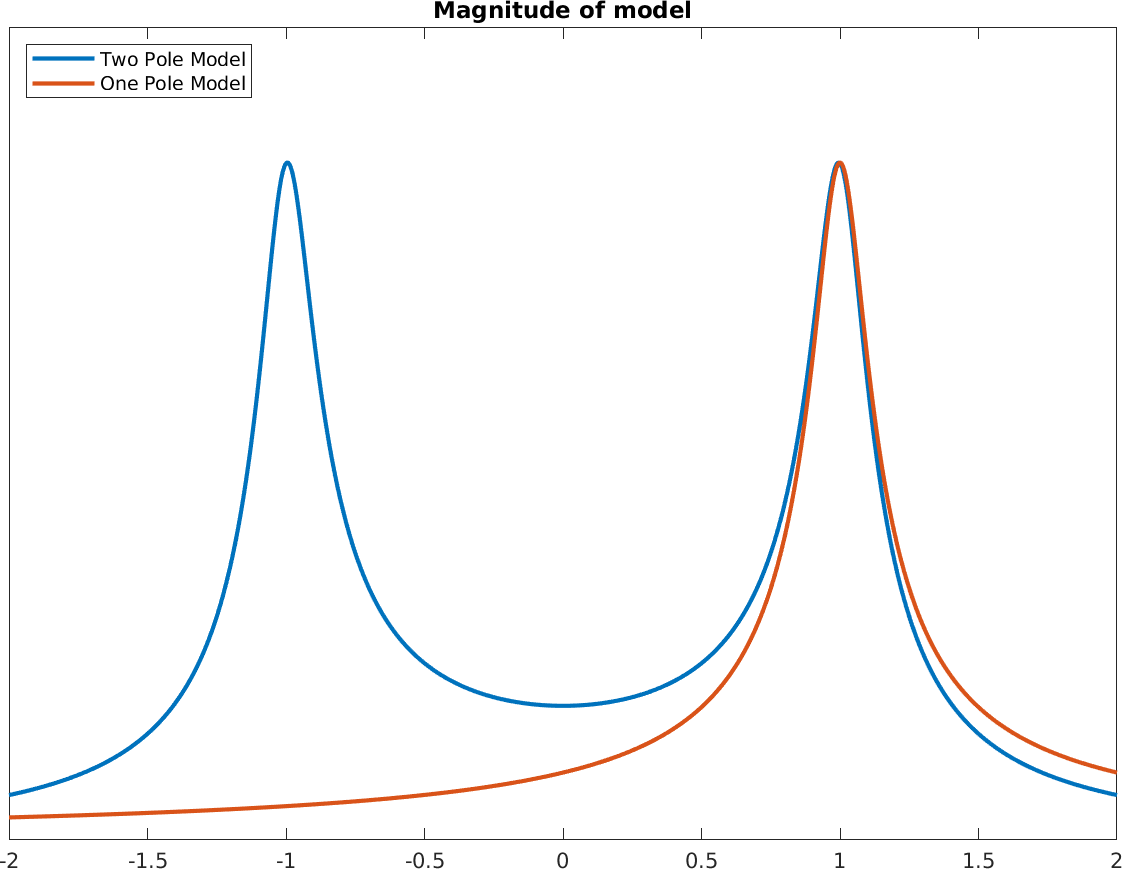
\includegraphics[width=\linewidth]{one-pole-model.png}
\end{minipage}
\quad
\begin{minipage}{0.50\textwidth}
Our measurements are very narrow band, and we only sweep a narrow range, so we
can ignore one pole:
\[
    M(\omega) = \frac XY(i\omega) \approx \frac{a}{i\omega-b}
    = \frac{a'}{\omega-b'}
\]
Result is a ``Single Pole Resonator'' model.

\bigskip
\scriptsize{Example Q is 10, typical tune Q is 100s to 1000s.}
\end{minipage}

\end{frame}


% ------------------------------------------------------------------------------
%
\begin{frame}{Multi-pole Resonator Model}

Modelling the raw data as a sum of one pole resonators produces a good fit to
experimental data:

\begin{center}
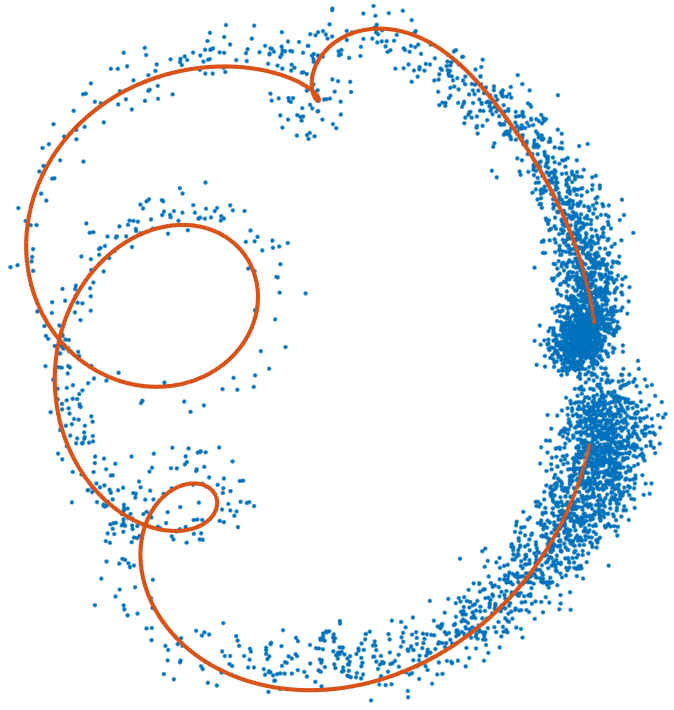
\includegraphics[align=c, width=0.25\linewidth]{good-raw-fit.png}
\qquad
$\displaystyle
    M(\omega) = \sum_{n=1}^N\frac{a_n}{\omega-b_n} + c
              = \frac{P(\omega)}{Q(\omega)}
$

\end{center}

\medskip

This is mathematically sound, produces a convincing fit when successful, but is
surprisingly tricky to fit numerically.

\end{frame}


% ------------------------------------------------------------------------------
%
\begin{frame}{Extracting Data From Model}

\begin{center}
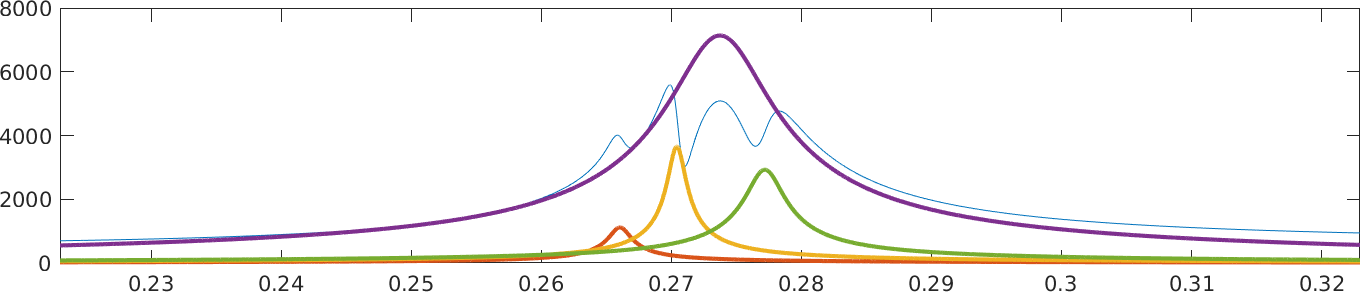
\includegraphics[width=0.8\linewidth]{good-peaks.png}
\end{center}

\def\arraystretch{1.2}
\begin{tabular}{l>{$\displaystyle}c<{$}ccccl}
 & $\cg Equation$ & \cg Peak -2 & \cg Peak -1 & \cg Tune & \cg Peak +1 \\
\cg Tune & \re(b) &
    0.2661 & 0.2704 & \cy 0.2737 & 0.2772 \\
\cg Width & \im(b) &
    0.9 & 0.7 & \cy 3.9 & 1.5 & ($\times10^{-3}$) \\
\cg ``Power'' & \int_\R|M(\omega)|^2\,d\omega = \frac{|a|^2}{\im(b)} &
    0.04 & 0.25 & \cy 1 & 0.5 & \footnote{Relative to tune power} \\
\cg Phase & \angle (i\cdot a) &
    170\textdegree & -110\textdegree & \cy 180\textdegree & 110\textdegree \\
\end{tabular}

\end{frame}


% ------------------------------------------------------------------------------
%
\begin{frame}{Algorithm}

We fit as many peaks as we can up to a configured number of peaks.
\begin{itemize}
\item Fit one peak at a time until done
\item Find largest peak in residual response power
\item Simple linear fit to discovered peak
\item Refine fit with non-linear optimisation
\item Assess quality of resulting model, discard and stop if poor
\end{itemize}
When fitting is done take peak with largest ``power'' as the tune.

\end{frame}


% ------------------------------------------------------------------------------
%
\begin{frame}{Peak Discovery}

\begin{minipage}{0.4\textwidth}
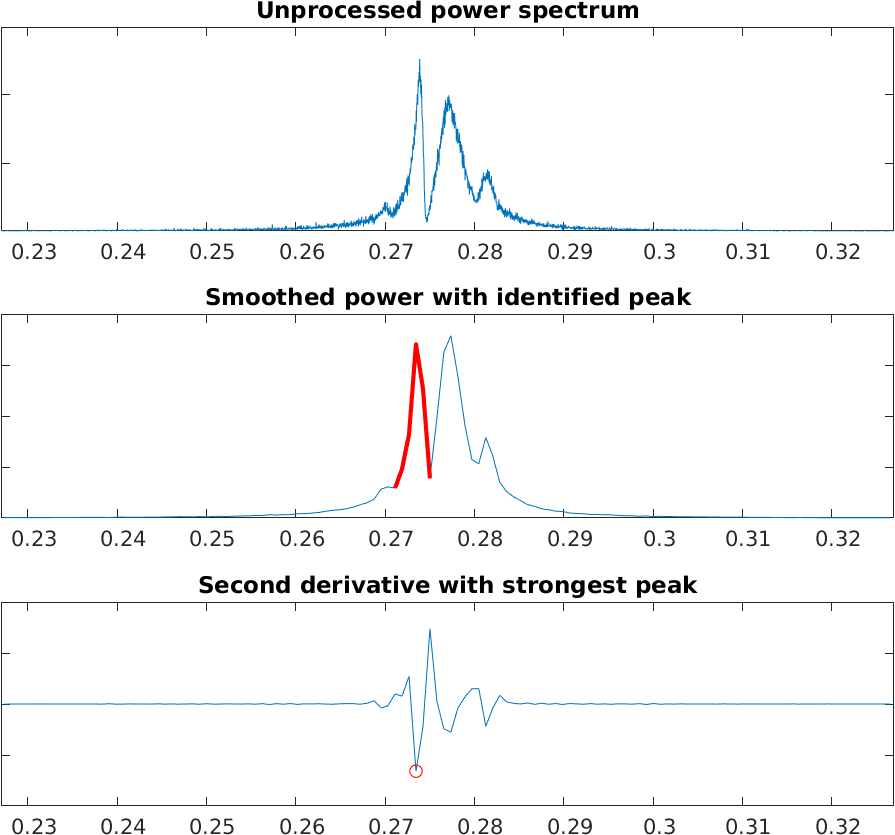
\includegraphics[width=\linewidth]{discover-peak.png}
\end{minipage}%
\quad
\begin{minipage}{0.55\textwidth}
\begin{itemize}
\item Compute residue by subtracting model so far from data to fit:
    \[
        r(\omega) = R(\omega) - M(\omega)
    \]
\item Smooth and decimate power $|r|^2$, take second derivative
    $d^2\mathcal{S}(|r|^2)/d\omega^2$.

\medskip

    Select point with
    largest curvature as peak: inspired by early computer vision methods!
\item Follow curve to define interval for initial fit.
\end{itemize}

This method tends to become brittle as more peaks are fitted.
\end{minipage}

\end{frame}


% ------------------------------------------------------------------------------
%
\begin{frame}{Overview of One Round of Fitting}

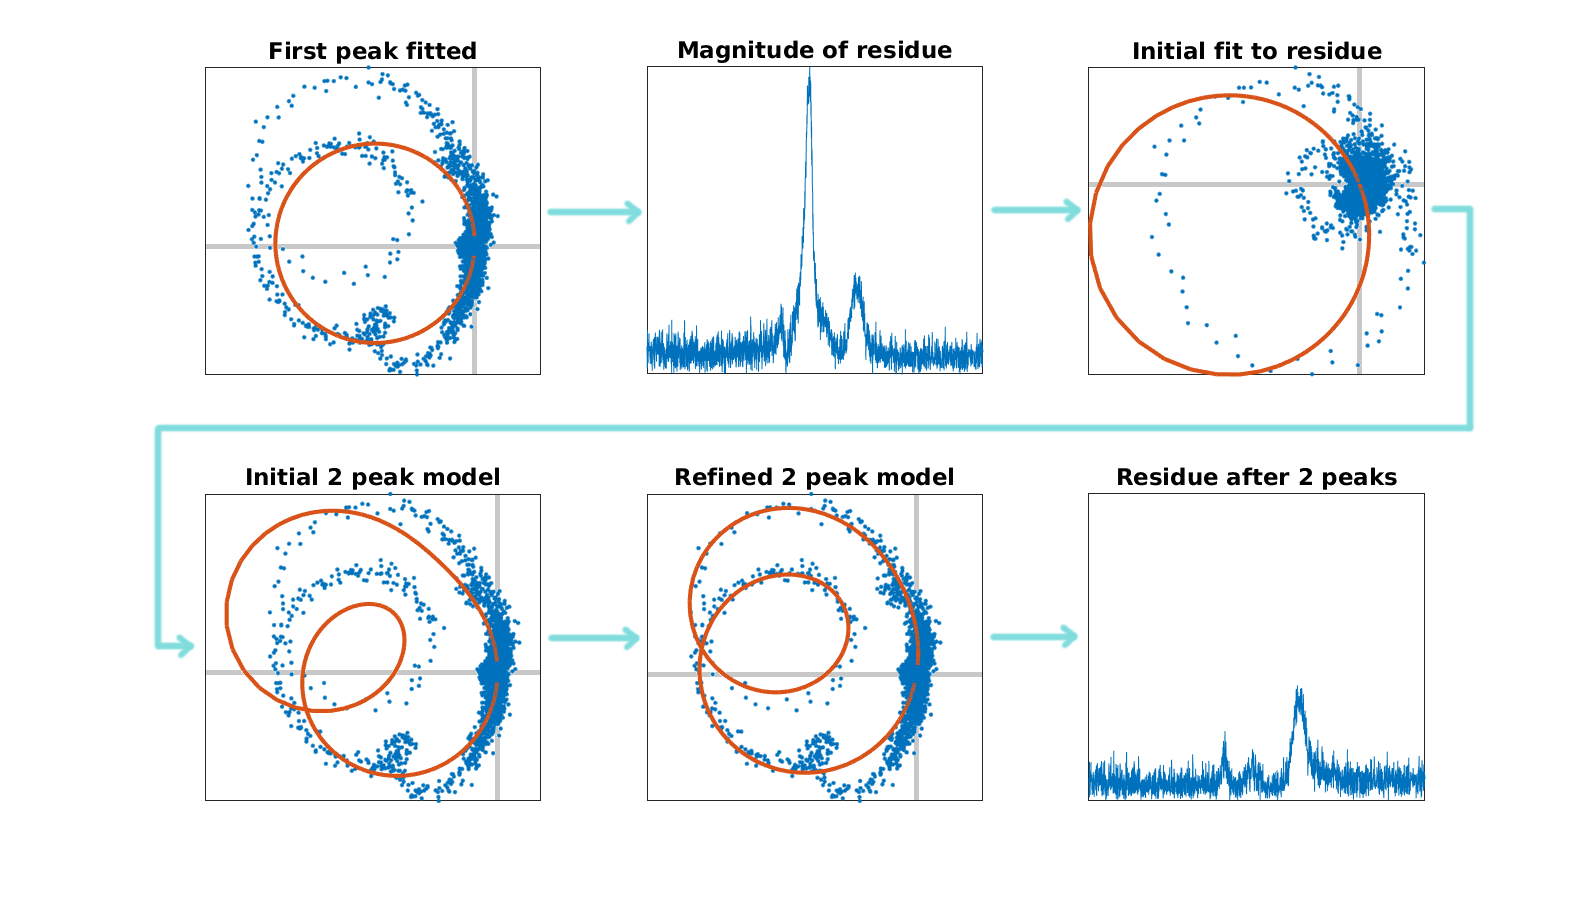
\includegraphics[width=\linewidth]{fit-and-refine.png}

\end{frame}


% ------------------------------------------------------------------------------
%
\begin{frame}{Fit Refinement}

Fit refinement is done using the Levenberg-Marquardt algorithm to optimise the
fit.

The figure below shows the impact of this step.

\medskip

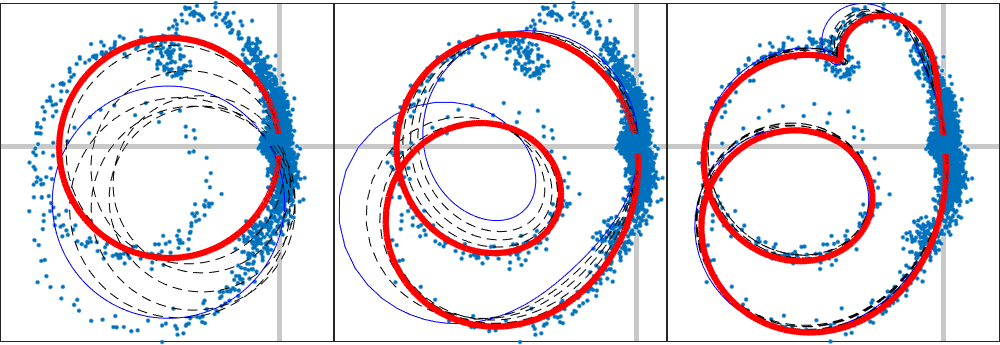
\includegraphics[width=\linewidth]{fit-refine.png}

Dots: data to fit;\quad thin blue line: initial model;\quad thick red line:
refined model.

\end{frame}


% ------------------------------------------------------------------------------
%
\begin{frame}{Challenges}

I will end with a few challenging fits.

\end{frame}


% ------------------------------------------------------------------------------
%
\begin{frame}{Sometimes it fits}

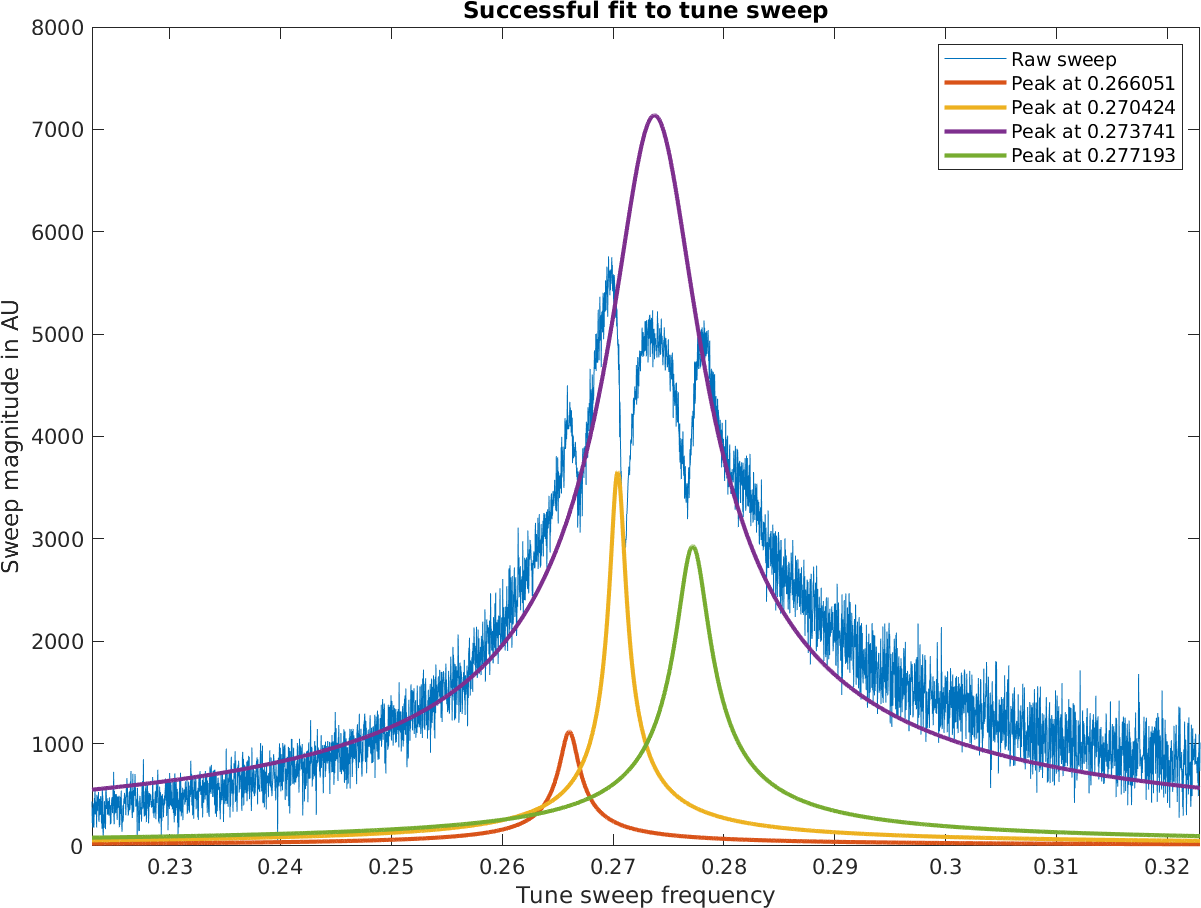
\includegraphics[width=0.45\linewidth]{hard-fit-ok.png}
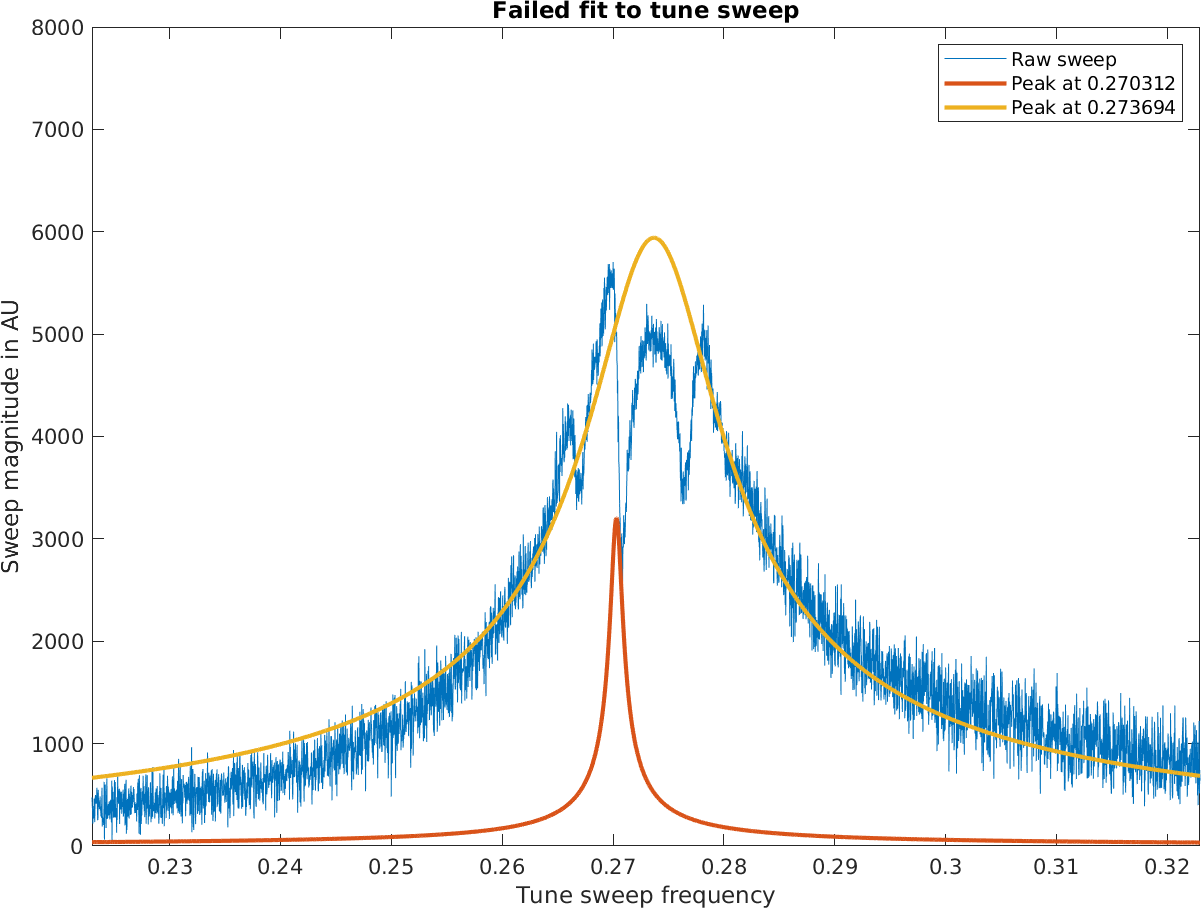
\includegraphics[width=0.45\linewidth]{hard-fit-fail.png}

Here we see two almost identical sweeps.  Perfect fit on the left, only two
peaks fitted on the right.  In this case we tried and failed to fit the smallest
peak next!

\end{frame}


% ------------------------------------------------------------------------------
%
\begin{frame}{ESRF: Vertical Tune}

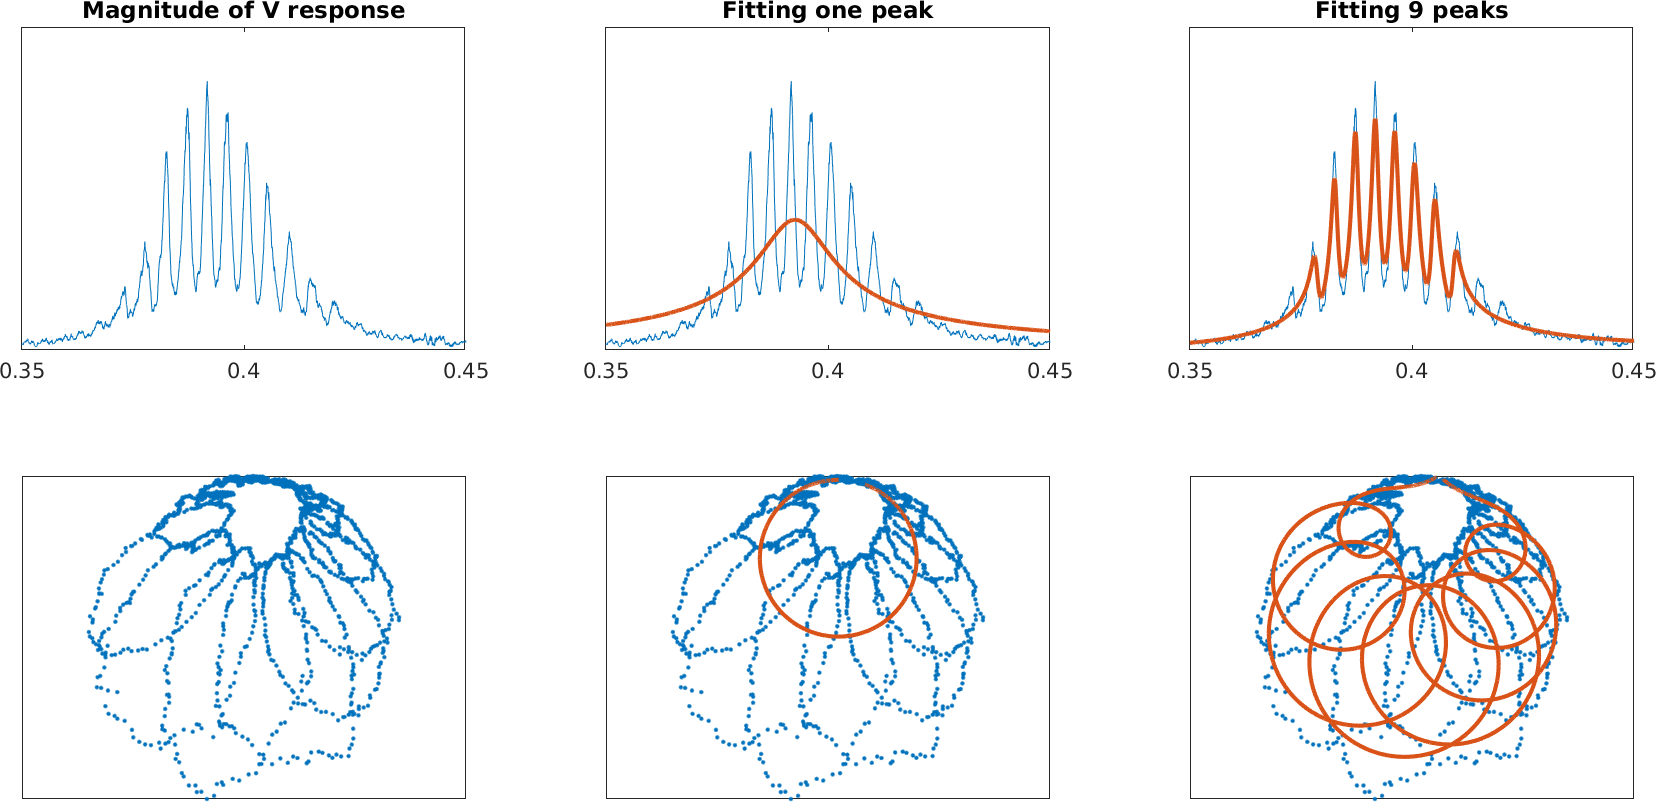
\includegraphics[width=\linewidth]{esrf-V.png}

\end{frame}


% ------------------------------------------------------------------------------
%
\begin{frame}{ESRF: Horizontal Tune}

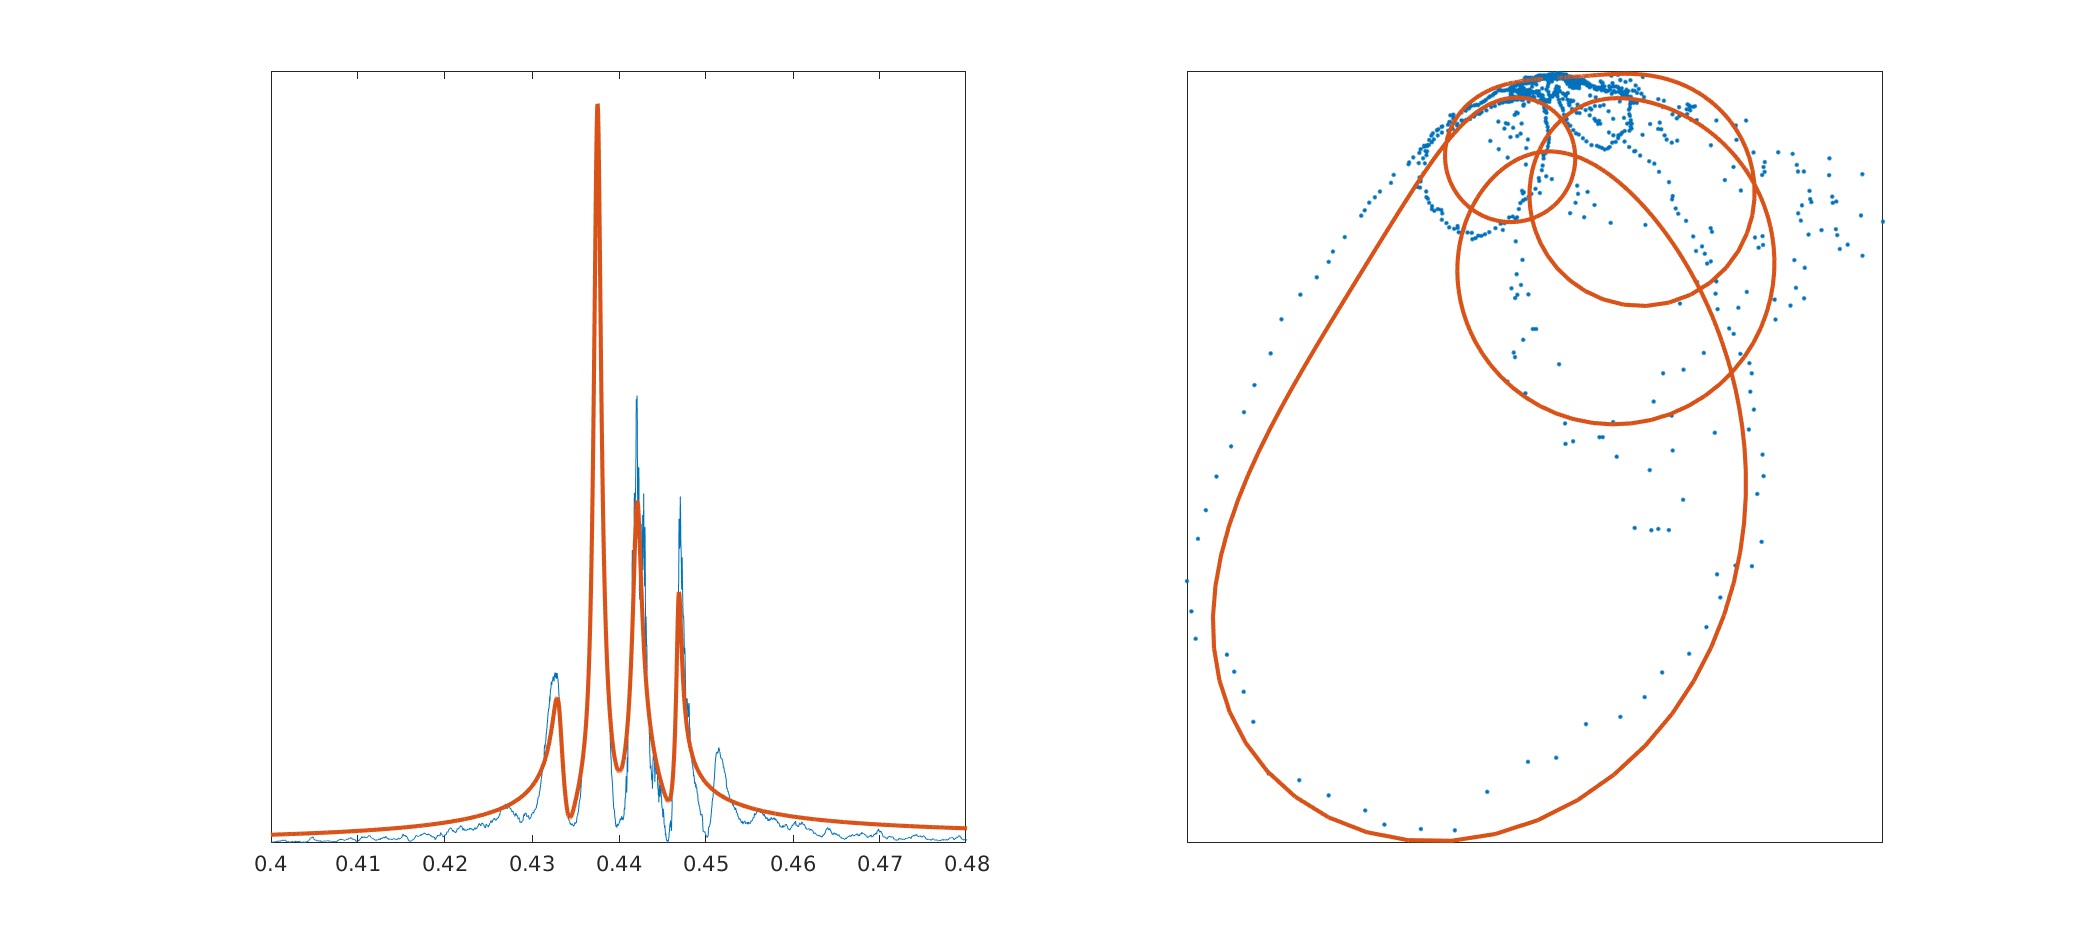
\includegraphics[width=\linewidth]{esrf-H.png}

\end{frame}


% ------------------------------------------------------------------------------
%
\begin{frame}{END}

\vfill
Extra slides follow.

\end{frame}


% ------------------------------------------------------------------------------
%
\begin{frame}{Wandering Peaks}

\raisebox{-0.5\height}{
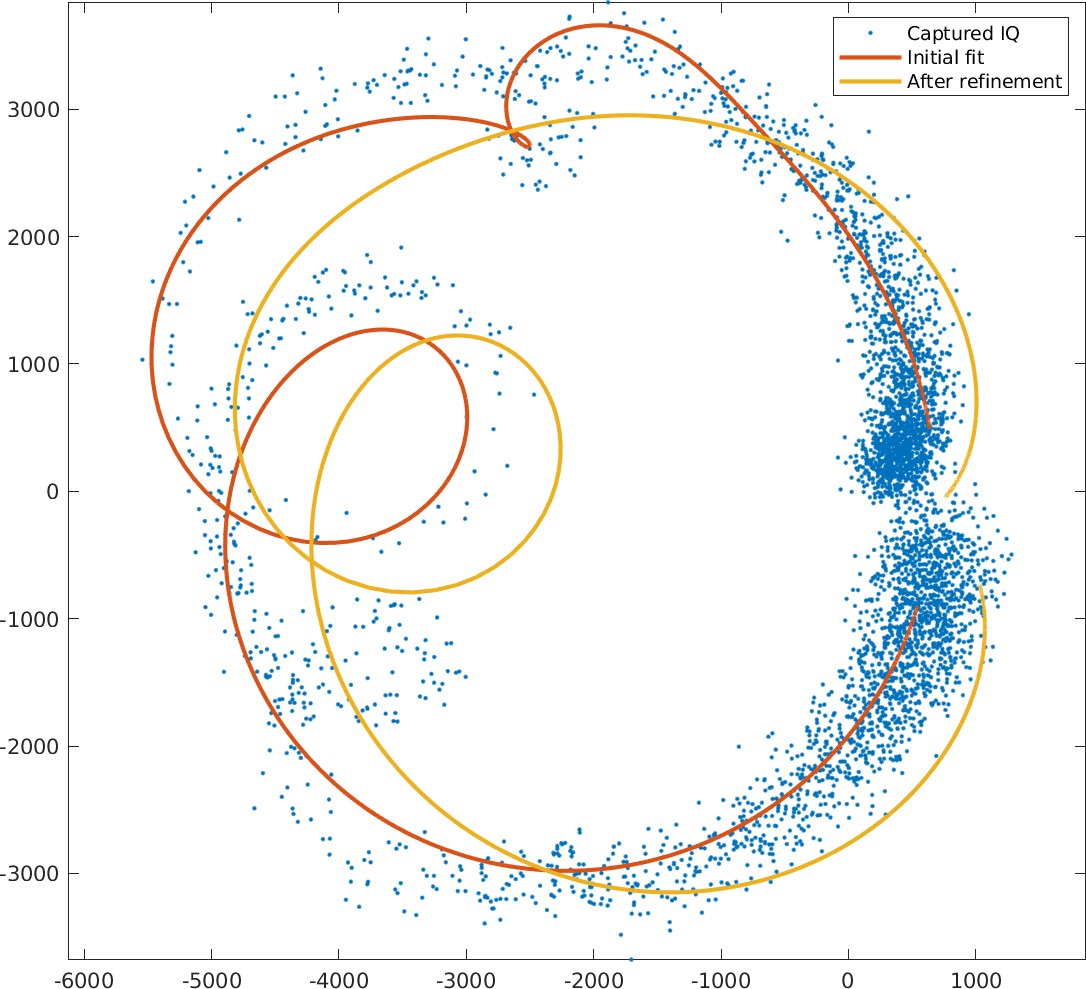
\includegraphics[width=0.45\linewidth]{hard-fit-fail-initial.png}}
\quad
\raisebox{-0.5\height}{
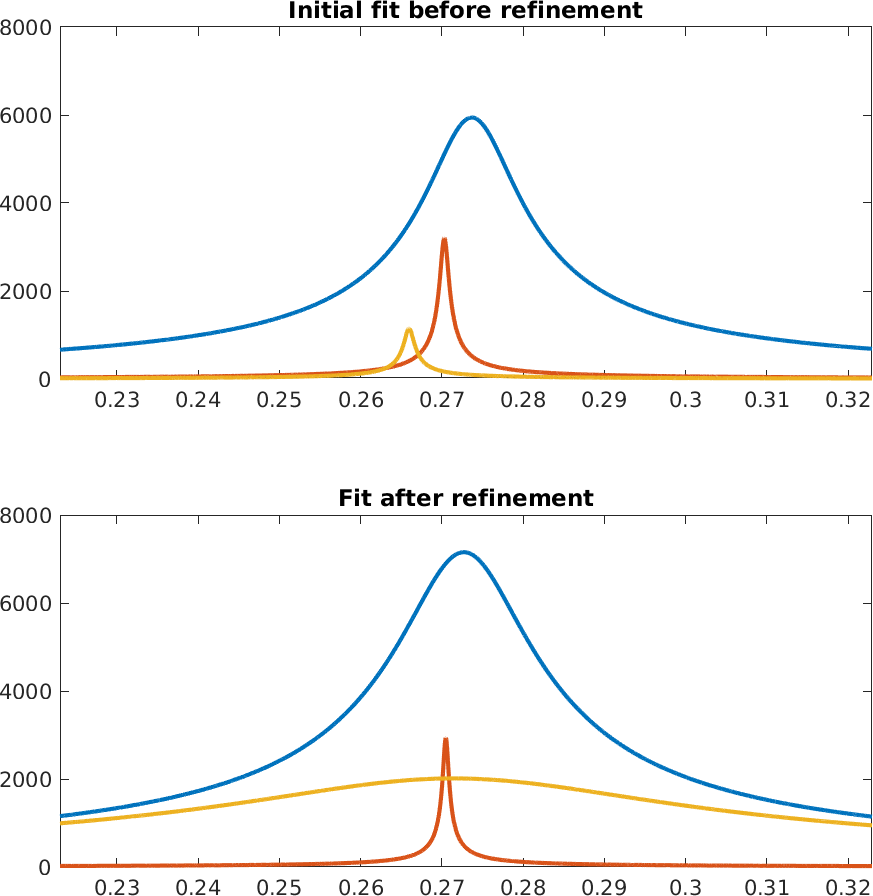
\includegraphics[width=0.45\linewidth]{hard-fit-fail-peaks.png}}


\end{frame}


% ------------------------------------------------------------------------------
%
\begin{frame}{Wandering During Refinement}

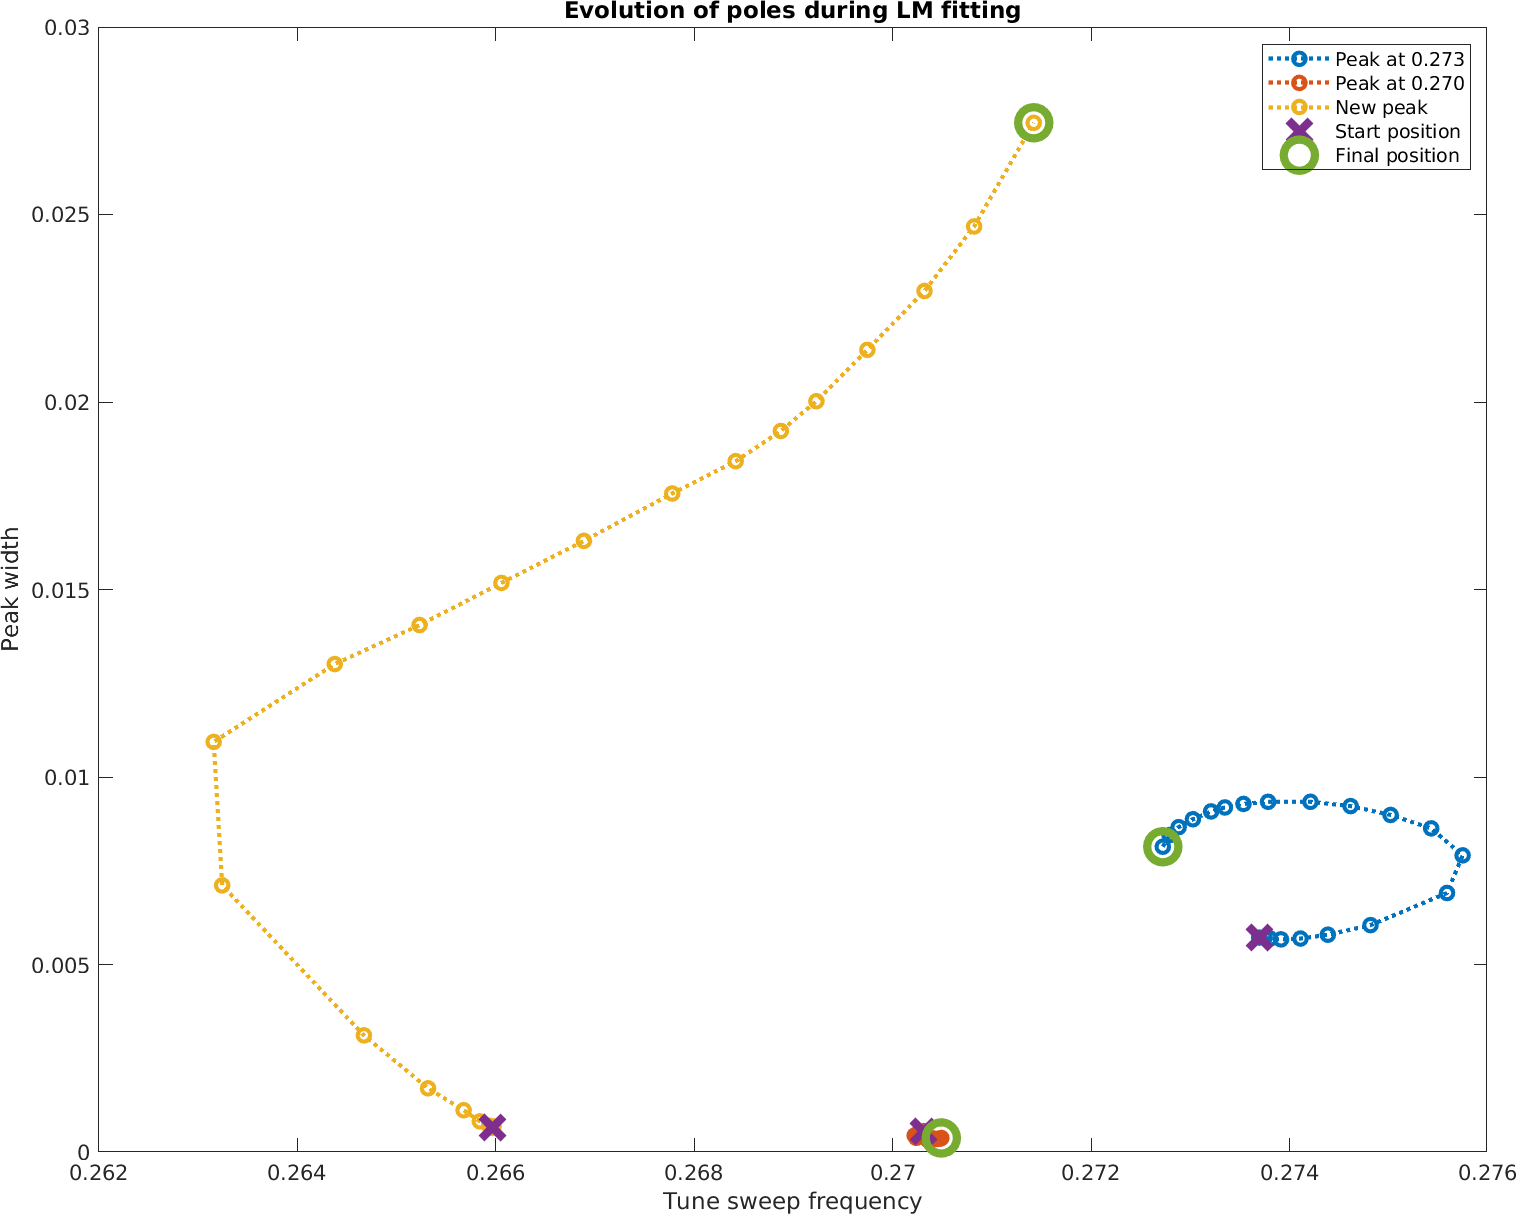
\includegraphics[width=0.48\linewidth]{hard-fit-fail-poles.png}
\quad
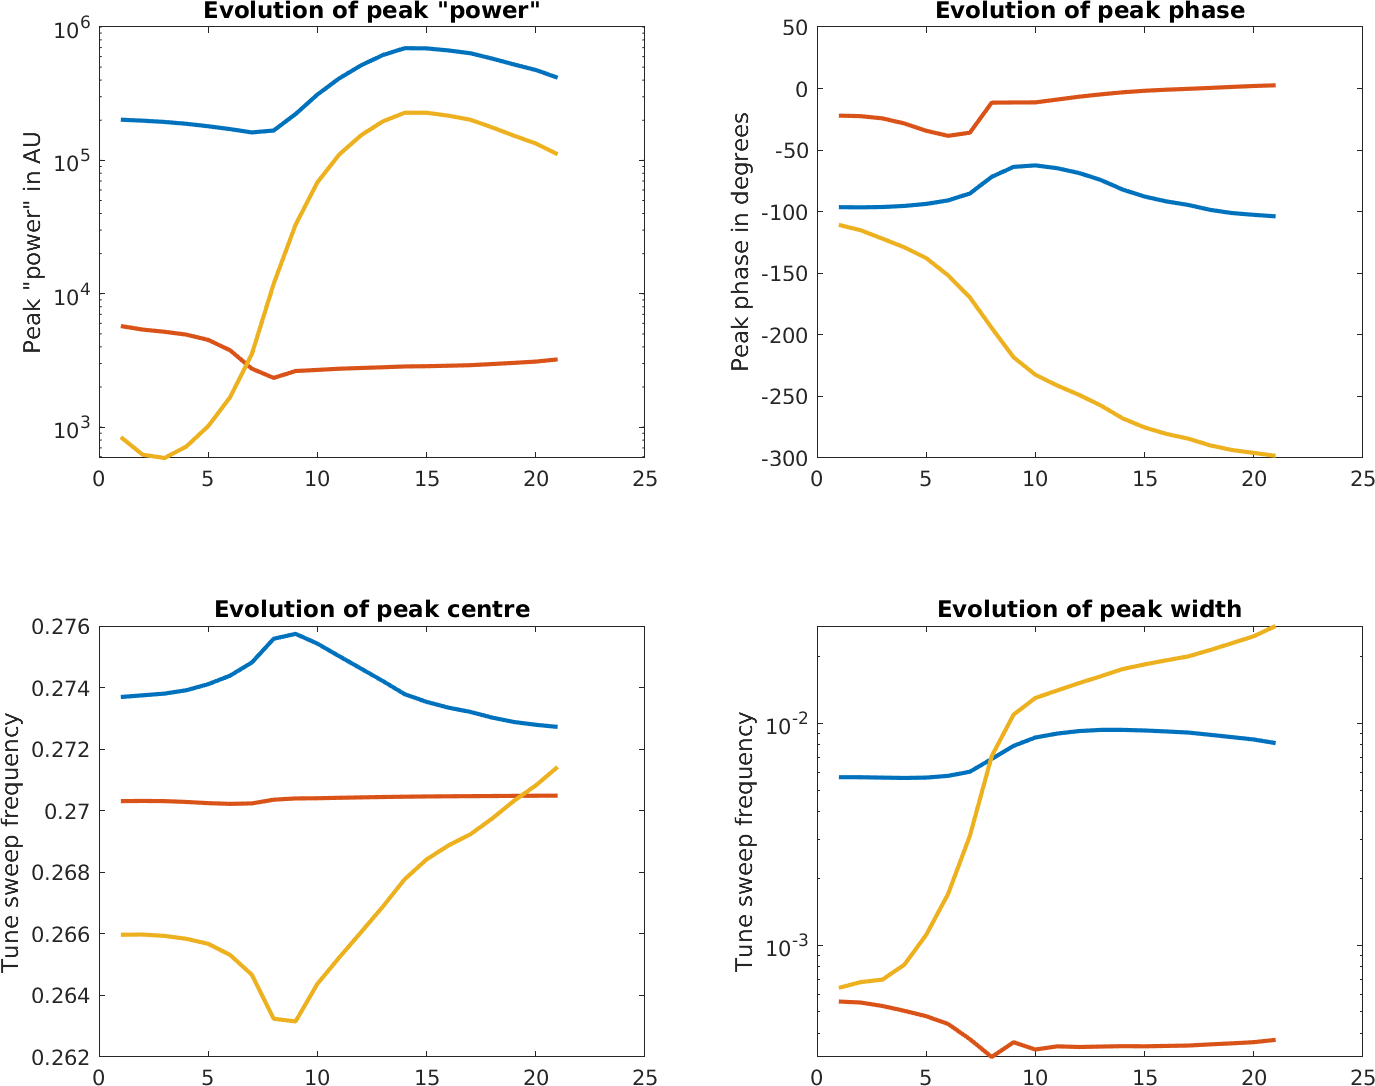
\includegraphics[width=0.48\linewidth]{hard-fit-fail-evolve.png}

\end{frame}


\end{document}


% ------------------------------------------------------------------------------
%
\begin{frame}{}


\end{frame}


